\chapter{Research Methodology}
\label{Chapter2} % For referencing this chapter elsewhere, use \ref{Chapter3}

\section{Research design} \label{design}
For the proposed research, a rigorous framework has been formalized by \parencite{morris_using_2019} and will be referred to as (ADMEP). As \parencite{morris_using_2019} states, "Simulation studies are used to obtain empirical results about the behavior of statistical methods in certain scenarios, as opposed to analytic results", which is at the foundation of the objectives of this research. In essence, this study aims to produce results that accurately represent the efficacy of the Random Survival Forest \parencite{ishwaran_random_2008} and the Cox proportional hazards model \parencite{cox_regression_1972}. 

\begin{figure}[h]
 \centering
 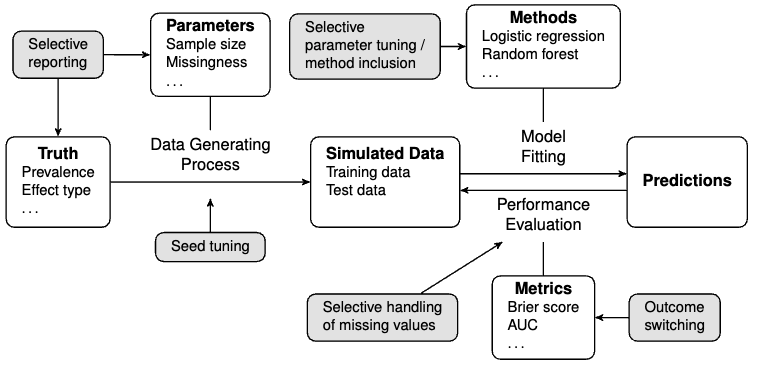
\includegraphics[scale=0.48]{Figures/METHOD_GRAPH.png}
 \caption{\parencite{pawel_pitfalls_2024} showing a common example of a simulation study.}
\end{figure}

\noindent Taking inspiration from the the application of ADMEP by \parencite{pawel_pitfalls_2024}, the following sections define the research broadly:

\subsection{Aims}
\begin{itemize} 
\item To evaluate how effectively the Random Survival Forest and Lasso-Cox models predict survival outcomes.
\item To understand model behavior under varying conditions of data complexity and censoring rates.
\end{itemize}

\subsection{Data-generating mechanisms}
\begin{itemize}
\item Simulate datasets with packages like \parencite{davidson-pilon_lifelines_2024} to introduce complexities like varying censoring rates and non-linear effects.
\item Introduce multicollinearity and various interaction effects to challenge the models' assumptions and robustness.
\item In case of spare time and ahead-of-schedule succesful implementation, explore individual survival distributions \parencite{haider_effective_2018}, as well as competing risk data \parencite{meng_simulating_2023}.
\end{itemize}

\subsection{Methods}
\begin{itemize}
\item Random Survival Forest: Implement using a combination of proposed packages in \ref{methods}, tuning tree-related parameters.
\item Lasso-Cox Model: Use a combination of the proposed packages in \ref{methods} for implementing Cox regression with Lasso regularization, optimizing the regularization strength and model complexity. 
\item Explore integration effects from the different packages.
\item In case of spare time and ahead-of-schedule successful implementation, explore adaptations of core methods.
\end{itemize}

\subsection{Estimands}
\begin{itemize}
\item Focus on estimations, like survival functions, hazard ratios, etc. for both models and survival probabilities at specified time points.
\item Analyze feature importance in RSF and assess how Lasso regularization affects the selection of covariates in the Cox model.
\item Bootstrap samples to build confidence intervals for key estimands, ensuring the robustness of the findings.
\end{itemize}

\subsection{Performance measures}
\begin{itemize}
\item Use statistical tests, like the C-index, and integrated Brier score as proposed in \ref{eval} to compare the RSF and Lasso-Cox model's performance metrics, like predictive accuracy and calibration across time.
\item Apply graphical methods like Kaplan-Meier curves to visualize survival estimates against actual outcomes.
\item Conduct sensitivity analysis to explore the impact of model parameters on their performance.
\end{itemize}

\section{Data}
\noindent The process of finding a dataset suitable for the study forms part of research execution. I will focus on sourcing data from reputable, well-established libraries such as UCI Machine Learning Repository, Kaggle, and available software libraries examples being, \parencite{nagpal_auton-survival_2022} \parencite{davidson-pilon_lifelines_2024} \parencite{sebastian_polsterl_scikit-survival_2023}. This approach guarantees access to a diverse array of well-documented datasets, ensuring both reliability and reproducibility of the results. It is important to note that the selection of data generation mechanisms (DGM), is indirectly dependent on the dataset chosen, so it is important to incorporate and accommodate the selection process toward ease of implementation of the DGM. Furthermore, when selecting the dataset censoring levels, FAIR principles \parencite{wilkinson_fair_2016}, reproducibility by assessing data simulation accuracy similar to the KM-Divergence metric used by \parencite{norcliffe_survivalgan_2023} are all important considerations. Utilizing this approach voids the need to carefully assess the ethical implications of using the datasets as these datasets should be under public licensed availability. Lastly, I don't foresee data preprocessing steps, being necessary, as DGM for simulation are commonly categorized as postprocessing \parencite{jin_imputation_2024}. 

\section{Methods} \label{methods}
I show a few widely used libraries within the field of survival analysis. The popularity of these libraries is qualitatively assessed based on metrics such as the number of GitHub stars, which serve as a proxy for community approval and usage frequency. Additionally, the maintenance history of these libraries is evaluated by examining the date of the most recent commit, providing insight into their current relevance and reliability. A detailed overview of these libraries is presented in the accompanying table, illustrating their prominence and role in both historical and contemporary research within the survival analysis space. To ensure robustness and interoperability in my research, I aim to adopt common software standards across different execution libraries. A notable example is the use of the pandas DataFrame object which is a very popular data structure. This will allow integration of various libraries, allowing for options across research phases (evaluation, model execution, etc.), and by standardizing data structures across different tools, I can minimize compatibility issues and streamline the process of switching between different analytical methods and environments.
\\\\
\noindent \begin{tabularx}{\textwidth}{|X|X|}
\hline
Library/Method & Description \\
\hline
Auton-survival \parencite{nagpal_auton-survival_2022} & Provides tools for survival analysis including implementations of advanced machine learning models like DeepSurv and Cox-Time. \\
\hline
scikit-survival \parencite{sebastian_polsterl_scikit-survival_2023} & Extends scikit-learn \parencite{scikit-learn} to handle survival analysis, enabling use of Cox regression models with extensions such as Lasso. \\
\hline
lifelines \parencite{davidson-pilon_lifelines_2024} & Popular library for survival analysis that includes Kaplan-Meier, Nelson-Aalen, and Cox models, among others. \\
\hline
pcoxtime \parencite{cygu_pcoxtime_2021} & Implements penalized Cox models with time-varying covariates in Python. \\
\hline
random-survival-forest \parencite{spath_julianspaethrandom-survival-forest_2021} & Implementation of Random Survival Forests that allows for detailed configuration and robust analysis. \\
\hline
\end{tabularx}
\\\\
\noindent I plan to use the above packages, or packages that might gain more popularity that were not investigated at the time of writing this document, to perform the comparative study between a random survival forest implementation and the lasso regularized Cox proportional hazards model, using simulated data according to the ADMEP research design proposal in \ref{design}

\section{Limitations}
A massive limitation is that the research is tightly coupled, meaning the phases are strictly dependent on each other. This is an antipattern, \parencite{joshi_beginning_2016}, which should be planned to accommodate any failures during any of the research phases. In cases where results do not converge, or the interpretation is wrong, the tightly coupled nature of the research will also affect the preceding stages. Lastly the computation time, within the modern setting should not be a hindrance but the combination of multiple computational components like the DGM and the model execution and results evaluation, is important to take caution. 

\section{Ethical Considerations}
Ethical clearance would not be a component of this study, as the only real data that would be used, will only be selected from open source, or publicly available (public licensing) sources. Due to the nature of the topic, being closely related to sensitive information, it will be an important point of order to note in the case that results indicate or underscore ethical implications.


